\begin{tabular}{M{6.5cm}M{11cm}}
	\textbf{LỚP CÔ THẢO - THẦY SANG}& \textbf{ĐỀ ÔN TẬP KIỂM TRA GIỮA HỌC KÌ 1}\\
	\textbf{MÃ ĐỀ: 002}& \textbf{Bài thi môn: VẬT LÝ 12}\\
	\textit{(Đề trường TH - THCS - THPT\newline Lê Thánh Tông năm 2024 -2025)}& \textit{Thời gian làm bài: 50 phút, không kể thời gian phát đề}
	
	\noindent\rule{4cm}{0.8pt} \\
\end{tabular}
\setcounter{section}{0}
\section{Câu trắc nghiệm nhiều phương án lựa chọn}
\textit{Thí sinh trả lời từ câu 1 đến câu 18. Mỗi câu hỏi thí sinh chọn một phương án}
\setcounter{ex}{0}
\Opensolutionfile{ans}[ans/G12-2-TN]
% ===================================================================
\begin{ex}
	Các vật không thể có nhiệt độ thấp hơn
	\choice
	{$\SI{2.0}{\kelvin}$}
	{$\SI{0}{\celsius}$}
	{$\SI{100}{\kelvin}$}
	{\True $\SI{-273.15}{\kelvin}$}
	\loigiai{}
\end{ex}
% ===================================================================
\begin{ex}
	Chọn câu đúng.	
	\choice
	{Khi một vật tỏa nhiệt ra môi trường thì nội năng của vật tăng lên}
	{Độ biến thiên nội năng của một vật là độ biến thiên nhiệt độ của vật đó}
	{\True Nội năng là phần năng lượng vật nhận được hay mất đi trong quá trình truyền nhiệt}
	{Nội năng của vật phụ thuộc vào nhiệt độ và thể tích của vật}
	\loigiai{}
\end{ex}
% ===================================================================
\begin{ex}
	Cho hai vật A và B tiếp xúc nhau. Nhiệt chỉ tự truyền từ A sang B khi
	\choice
	{A và B là hai vật rắn}
	{nhiệt độ của A và của B bằng nhau}
	{\True nhiệt độ của A lớn hơn nhiệt độ của B}
	{khối lượng của A lớn hơn khối lượng của B}
	\loigiai{}
\end{ex}
% ===================================================================
\begin{ex}
	Phát biểu nào dưới đây nói về nhiệt lượng là \textbf{không đúng}?	
	\choice
	{Nhiệt lượng là số đo độ biến thiên nội năng của vật trong quá trình truyền nhiệt}
	{\True Một vật lúc nào cũng có nội năng, do đó lúc nào cũng có nhiệt lượng}
	{Nhiệt lượng không phải là nội năng}
	{Đơn vị của nhiệt lượng cũng là đơn vị của nội năng}
	\loigiai{}
\end{ex}
% ===================================================================
\begin{ex}
	Trong quá trình chất khí nhận nhiệt lượng $Q$ và sinh công $A$, nội năng của một lượng khí biến thiên một lượng $\Delta U=A+Q$. Khi đó, $A$ và $Q$ phải thỏa mãn điều kiện nào dưới đây?
	\choice
	{$Q<0$ và $A>0$}
	{$Q<0$ và $A<0$}
	{\True $Q>0$ và $A<0$}
	{$Q>0$ và $A>0$}
	\loigiai{}
\end{ex}
% ===================================================================
\begin{ex}
	Câu nào sau đây nói về nội năng là \textbf{không đúng}?
	\choice
	{Nội năng của một hệ có thể tăng lên hoặc giảm xuống}
	{Nội năng là một dạng năng lượng}
	{Nội năng có thể chuyển hóa thành các dạng năng lượng khác}
	{\True Nội năng là nhiệt lượng}
	\loigiai{}
\end{ex}
% ===================================================================
\begin{ex}
	Chọn câu đúng.\\ 
	Trong quá trình hóa hơi một lượng chất lỏng ở nhiệt độ sôi
	\choice
	{\True nhiệt độ chất lỏng không thay đổi}
	{thể tích khối chất lỏng không thay đổi}
	{nhiệt độ của chất lỏng tăng liên tục}
	{nhiệt độ của chất lỏng giảm liên tục}
	\loigiai{}
\end{ex}
% ===================================================================
\begin{ex}
	Trong quá trình nóng chảy của nước đá đến khi nóng chảy hoàn toàn thì nhiệt độ của nước đá	
	\choice
	{tăng lên sau đó giảm xuống}
	{\True không thay đổi}
	{luôn giảm}
	{luôn tăng}
	\loigiai{}
\end{ex}
% ===================================================================
\begin{ex}
	Nếu làm tăng nhiệt độ của một hệ mà không làm thay đổi thể tích của nó thì nội năng của hệ sẽ
	\choice
	{\True tăng lên}
	{không thay đổi}
	{giảm xuống}
	{tăng lên sau đó giảm xuống}
	\loigiai{}
\end{ex}
% ===================================================================
\begin{ex}
	Phần năng lượng nhiệt mà vật này truyền cho vật kia hoặc vật này nhận từ vật kia gọi là	
	\choice
	{nội năng.}
	{thế năng}
	{nhiệt độ}
	{\True nhiệt lượng}
	\loigiai{}
\end{ex}
% ===================================================================
\begin{ex}
	Trường hợp nào dưới đây làm biến đổi nội năng \textbf{không phải} do thực hiện công?	
	\choice
	{Cọ xát hai vật vào nhau}
	{Nén khí trong xilanh}
	{\True Đun nóng nước bằng bếp}
	{Một viên bi bằng thép rơi xuống đất mềm}
	\loigiai{}
\end{ex}
% ===================================================================
\begin{ex}
	\immini{
		Hình bên là đường biểu diễn sự thay đổi nhiệt độ theo thời gian khi làm lạnh nước tinh khiết. Nhận định nào dưới đây là đúng?
		\choice
		{\True Từ phút thứ 5 tến phút thứ 6, nước ở cả thể lỏng và thể rắn}
		{Từ phút thứ nhất đến phút thứ hai, nước ở thể rắn}
		{Từ phút thứ 2 đến phút thứ 10 , nhiệt độ của nước không đổi}
		{Nhiệt độ của nước giảm đều theo thời gian}
	}
	{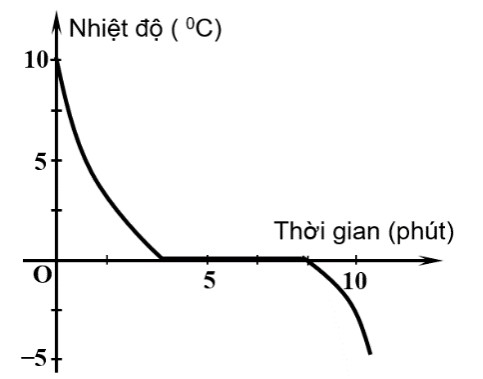
\includegraphics[width=0.6\linewidth]{../figs/D12-1-1}}
	\loigiai{}
\end{ex}
% ===================================================================
\begin{ex}
	Chiều cao của cột thủy ngân trong nhiệt kế thủy ngân thay đổi theo nhiệt độ. Ứng với hai vạch có nhiệt độ là $\SI{0}{\celsius}$ và $\SI{100}{\celsius}$ thì chiều cao của cột thủy ngân trong nhiệt kế là $\SI{2}{\centi\meter}$ và $\SI{22}{\centi\meter}$. Khi sử dụng nhiệt kế này để đo nhiệt độ của cơ thể của một em bé đang bị sốt thì thấy cột thủy ngân cao $\SI{9.9}{\centi\meter}$. Theo thang nhiệt Kelvin, nhiệt độ của em bé lúc này là bao nhiêu?
	\choice
	{$\SI{321.5}{\kelvin}$}
	{$\SI{305.5}{\kelvin}$}
	{$\SI{327.0}{\kelvin}$}
	{\True $\SI{312.5}{\kelvin}$}
	\loigiai{
		$$\dfrac{\ell -\ell_{\text{min}}}{\ell_{\text{max}}-\ell_{\text{min}}}=\dfrac{t -t_{\text{min}}}{t_{\text{max}}-t_{\text{min}}}\Leftrightarrow \dfrac{9,9-2}{22-2}=\dfrac{t-0}{100-0}\Rightarrow t=\SI{39.5}{\celsius}=\SI{312.5}{\kelvin}.$$
	}
\end{ex}
% ===================================================================
\begin{ex}
	Một viên đạn đại bác có khối lượng $\SI{10}{\kilogram}$ khi rơi tới đích có vận tốc $\SI{54}{\kilo\meter/\hour}$. Nếu toàn bộ động năng của nó biến thành nội năng thì nhiệt lượng tỏa ra lúc va chạm vào khoảng
	\choice
	{$\SI{14580}{\joule}$}
	{$\SI{2250}{\joule}$}
	{\True $\SI{1125}{\joule}$}
	{$\SI{7290}{\joule}$}
	\loigiai{
		$Q=\dfrac{1}{2}mv^2=\SI{1125}{\joule}$.
	}
\end{ex}
% ===================================================================
\begin{ex}
	Khi đun nóng một khối khí, khí giãn nở làm thể tích tăng thêm 7 lít. Biết trong quá trình này nội năng của khí giảm $\SI{1.1}{\kilo\joule}$ nhưng áp suất không đổi và bằng $\SI{3E5}{\pascal}$. Nhiệt lượng mà khối khí nhận được trong quá trình này là
	\choice
	{$\SI{3.2}{\kilo\joule}$}
	{\True $\SI{1.0}{\kilo\joule}$}
	{$\SI{1.5}{\kilo\joule}$}
	{$\SI{2.7}{\kilo\joule}$}
	\loigiai{
		Công khí thực hiện:
		$$A'=p\Delta V=\SI{2.1}{\kilo\joule}.$$
		Nhiệt lượng mà khối khí nhận được:
		$$Q=\Delta U-A=\Delta U+A'=-1,1+2,1=\SI{1.0}{\kilo\joule}.$$
	}
\end{ex}
% ===================================================================
\begin{ex}
	Hình bên là dự báo thời tiết ở thành phố Hồ Chí Minh ngày 21/07/2024. Theo thang nhiệt Kelvin, nhiệt độ cao nhất và thấp nhất theo bảng dự báo bên là
	\begin{center}
		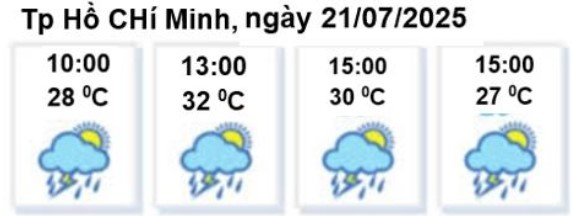
\includegraphics[width=0.3\linewidth]{../figs/D12-1-2}
	\end{center}
	\choice
	{$\SI{246}{\kelvin}$ và $\SI{241}{\kelvin}$}
	{\True $\SI{305}{\kelvin}$ và $\SI{300}{\kelvin}$}
	{$\SI{248}{\kelvin}$ và $\SI{236}{\kelvin}$}
	{$\SI{321}{\kelvin}$ và $\SI{306}{\kelvin}$}
	\loigiai{}
\end{ex}
% ===================================================================
\begin{ex}
	Một nhiệt kế có phạm vi đo từ $\SI{263}{\kelvin}$ đến $\SI{1273}{\kelvin}$, dùng để đo nhiệt độ của các lò nung. Phạm vi đo của nhiệt kế này trong thang nhiệt độ Celsius là
	\choice
	{$\SI{0}{\celsius}$ đến $\SI{273}{\celsius}$}
	{$\SI{-20}{\celsius}$ đến $\SI{1200}{\celsius}$}
	{\True $\SI{-10}{\celsius}$ đến $\SI{1000}{\celsius}$}
	{$\SI{-12}{\celsius}$ đến $\SI{1000}{\celsius}$}
	\loigiai{}
\end{ex}
% ===================================================================
\begin{ex}
	Khi nung nóng một lượng không khí chứa trong một xi lanh, khối khí nhận một nhiệt lượng $\SI{1.75}{\kilo\joule}$ làm nội năng của khí tăng thêm $\SI{720}{\joule}$. Khí giãn nở và sinh công làm pít - tông dịch chuyển. Khối khí đã thực hiện một công là	
	\choice
	{$\SI{2.56}{\kilo\joule}$}
	{\True $\SI{1.03}{\kilo\joule}$}
	{$\SI{1.25}{\kilo\joule}$}
	{$\SI{2.47}{\kilo\joule}$}
	\loigiai{
		$$A=\Delta U-Q=\SI{0.72}{\kilo\joule}-\SI{1.75}{\kilo\joule}=\SI{-1.03}{\kilo\joule}.$$
		Công khối khí thực hiện là $\SI{1.03}{\kilo\joule}$.
	}
\end{ex}
\Closesolutionfile{ans}
\section{Câu trắc nghiệm đúng/sai} 
\textit{Thí sinh trả lời từ câu 1 đến câu 4. Trong mỗi ý \textbf{a)}, \textbf{b)}, \textbf{c)}, \textbf{d)} ở mỗi câu, thí sinh chọn đúng hoặc sai}
\setcounter{ex}{0}
\Opensolutionfile{ans}[ans/G12-2-TF]
% ===================================================================
\begin{ex}
	Khi làm thí nghiệm đun nóng một chất. Kết quả thí nghiệm, một học sinh vẽ được biểu diễn sự thay đổi nhiệt độ của chất đó theo thời gian như hình bên.
	\begin{center}
		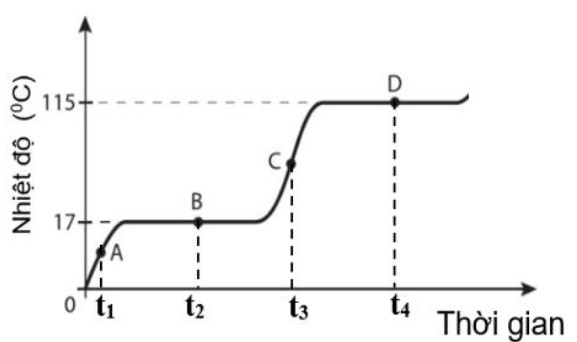
\includegraphics[width=0.4\linewidth]{../figs/D12-1-3}
	\end{center}
	\choiceTF[t]
	{Tại thời điểm $t_{2}$, chất ở thể lỏng}
	{\True Nhiệt độ nóng chảy của chất là $\SI{17}{\celsius}$}
	{Tại thời điểm $t_{3}$, chất ở thể rắn và thể lỏng}
	{\True Nhiệt độ sôi của chất này là $\SI{115}{\celsius}$}
	\loigiai{}
\end{ex}
% ===================================================================
\begin{ex}
	Có hai cốc nước A và B chứa cùng một lượng nước ở nhiệt độ phòng. Người ta thả một viên nước đá vào cốc A và nhúng cốc B vào một bình chứa nước nóng.
	\choiceTF[t]
	{\True Cốc B nhận nhiệt lượng từ nước ở bình, và nhiệt độ nước trong cốc tăng lên}
	{Nhiệt độ nước ở cốc A giảm vì nhận nhiệt lượng từ nước đá}
	{Nhiệt lượng không thể tự truyền từ nước ở cốc B vào nước ở bình chứa nó}
	{\True Khi nhiệt độ nước ở cốc B là $t_{2}=\SI{62}{\celsius}$ (theo thang nhiệt Celsius) thì theo thang nhiệt Kelvin là $T_{2} \approx \SI{335}{\kelvin}$}
	\loigiai{}
\end{ex}
% ===================================================================
\begin{ex}
	Đốt nóng khối khí trong xi lanh đặt nằm ngang bằng ngọn lửa đèn cồn như hình vẽ. Khí giãn nở đẩy pít - tông từ vị trí (1) đến vị trí (2).
	\begin{center}
		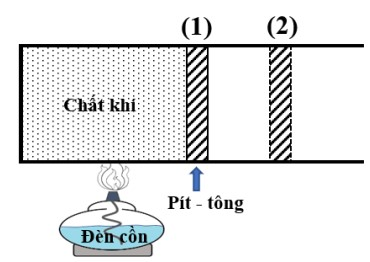
\includegraphics[width=0.3\linewidth]{../figs/D12-1-4}
	\end{center}
	\choiceTF[t]
	{\True Khối khí trong xi lanh nhận nhiệt lượng $Q\ (Q>0)$}
	{Khí dãn nở và nhận công $A\ (A>0)$}
	{\True Nội năng của khối khí khi pít - tông ở vị trí (2) là $\Delta U=Q+A$}
	{\True Khi khối khí trong xi lanh nhận được một nhiệt lượng $\SI{150}{\joule}$ thì khối khí giãn nở làm thể tích tăng từ $\SI{20}{\centi\meter^3}$ đến $\SI{30}{\centi\meter^3}$, biết rằng áp suất của khối khí trong xilanh không đổi và bằng $\SI{5E5}{\pascal}$. Nội năng của khối khí trong quá trình này tăng $\SI{145}{\joule}$}
	\loigiai{}
\end{ex}
% ===================================================================
\begin{ex}
	Các hình dưới đây là các đồ thị biểu diễn sự thay đổi thể tích $V$ phụ thuộc vào nhiệt độ $\left(\xsi{t}{\celsius}\right)$ trong quá trình nóng chảy của chì (H.1), của nước đá (H.2) và của sáp (nến) (H.3).	
	\begin{center}
		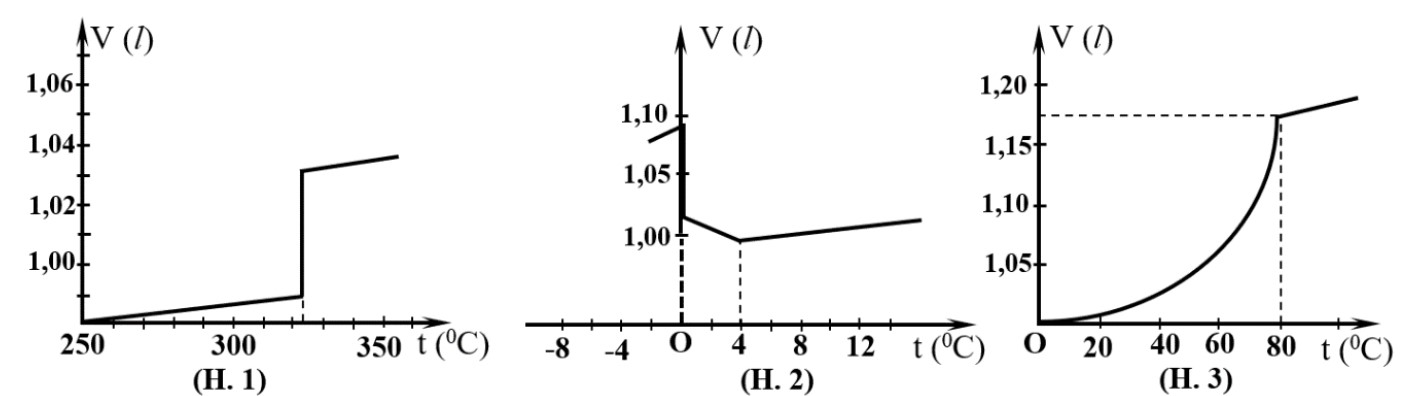
\includegraphics[width=0.9\linewidth]{../figs/D12-1-5}
	\end{center}
	\choiceTF[t]
	{Chì, nước đá và sáp (nến) đều có các nhiệt độ nóng chảy tương ứng nhất định}
	{Trong quá trình nóng chảy của chì, nước đá và sáp (nến) thể tích của chúng đều tăng tỉ lệ thuận với nhiệt độ}
	{\True Trong quá trình nóng chảy, nhiệt độ của chì và nước đá không thay đổi, còn nhiệt độ của sáp thay đổi liên tục}
	{\True Khi nóng chảy, chì và sáp (nến) dãn nở (thể tích $V$ tăng) còn nước đá co lại (thể tích $V$ giảm)}
	\loigiai{}
\end{ex}
\Closesolutionfile{ans}
\section{Câu trắc nghiệm trả lời ngắn} \textit{Thí sinh trả lời từ câu 1 đến câu 6}
\setcounter{ex}{0}
\Opensolutionfile{ans}[ans/G12-2-TL]
% ===============================================================
\begin{ex}
	Một lượng khí nhận một nhiệt lượng $\SI{35.40}{\kilo\joule}$ do được đun nóng, khí giãn ra và thực hiện một công $\SI{20.00}{\kilo\joule}$ ra môi trường xung quanh. Nội năng của khối khí này đã biến thiên một lượng bao nhiêu kilo joule $\left(\si{\kilo\joule}\right)$? \textit{(Kết quả lấy đến một chữ số sau dấu phẩy thập phân)}.	
	\shortans{15,4 }
	\loigiai{
		$\Delta U=Q+A=\SI{35.40}{\kilo\joule}-\SI{20.00}{\kilo\joule}=\SI{15.40}{\kilo\joule}$.
	}
\end{ex}
% ===============================================================
\begin{ex}
	Trong khoảng thời gian 2 phút 12 giây, nhiệt độ của một vật tăng từ $\SI{-15}{\celsius}$ đến $\SI{8.6}{\celsius}$. Nhiệt độ trung bình trong khoảng thời gian nói trên đã tăng bao nhiêu Kelvin/giây $\left(\si{\kelvin/\second}\right)$. \textit{(Kết quả lấy đến hai chữ số sau dấu phẩy thập phân)}.
	\shortans{0,33}
	\loigiai{
		$\dfrac{\Delta T}{\Delta t}=\dfrac{\SI{23.6}{\kelvin}}{\SI{72}{\second}}=\SI{0.33}{\kelvin/\second}.$
	}
\end{ex}
% ===============================================================
\begin{ex}
	Một khối khí được cung cấp nhiệt lượng $\SI{4.98}{\kilo\joule}$, khí giãn nở làm tăng thể tích một lượng $\xsi{\Delta V}{\deci\meter^3}$. Trong quá trình này, nội năng của khối khí biến thiên $\SI{1.23}{\kilo\joule}$ nhưng áp suất của khối khí không đổi và bằng $p=\SI{2.5E5}{\pascal}$. Giá trị của $\Delta \mathrm{V}$ là bao nhiêu?	
	\shortans{15 }
	\loigiai{
		$\Delta U=Q-p\Delta V\Rightarrow \Delta V=\SI{0.015}{\meter^3}=\SI{15}{\deci\meter^3}$.
	}
\end{ex}
% ===============================================================
\begin{ex}
	Một vật có khối lượng $\SI{2}{\kilogram}$ trượt không vận tốc đầu từ đỉnh xuống chân một mặt nghiêng dài $\SI{40}{\meter}$, nghiêng một góc $\SI{60}{\degree}$ so với phương ngang. Tốc độ của vật ở chân mặt phẳng nghiêng là $\SI{4.5}{\meter/\second}$. Cho rằng, $\SI{75}{\percent}$ công của lực ma sát giữa mặt phẳng nghiêng và vật chuyển thành nội năng của vật, bỏ qua phần nhiệt lượng mặt phẳng nghiêng truyền cho vật. Lấy $g=\SI{9.8}{\meter/\second^2}$. Độ biến thiên nội năng của vật trong quá trình trên là bao nhiêu kilo joule $\left(\si{\kilo\joule}\right)$. \textit{(Kết quả lấy đến hai chữ số sau dấu phẩy thập phân)}.
	\shortans{0,49 }
	\loigiai{
		$h=\ell\sin\alpha=\xsi{20\sqrt{3}}{\meter}$.\\
		Công lực ma sát:
		$$\left|A_{\text{ms}}\right|=W_1-W_2=mgh-\dfrac{1}{2}mv^2\approx\SI{658.7}{\joule}.$$
		Độ biến thiên nội năng của vật:
		$$\Delta U=0,75\left|A_{\text{ms}}\right|\approx\SI{0.49}{\kilo\joule}.$$
	}
\end{ex}
% ===============================================================
\begin{ex}
	Một xi lanh có pít - tông nằm ngang như hình vẽ, xilanh chứa $\SI{500}{\centi\meter^3}$ không khí. Khi đốt nóng khí trong xi lanh, khí giãn nở đẩy pít - tông qua phải làm thể tích khối khí tăng lên $\SI{720}{\centi\meter^3}$, nội năng khối khí tăng thêm $\SI{1.5}{\kilo\joule}$. Cho rằng áp suất của khối khí luôn bằng $5,8 \cdot 10^{5} \mathrm{~Pa}$. Nhiệt lượng đã cung cấp cho khối khí bao nhiêu kilôjun (kJ). \textit{(Kết quả lấy đến hai chữ số sau dấu phẩy thập phân)}.
	\begin{center}
		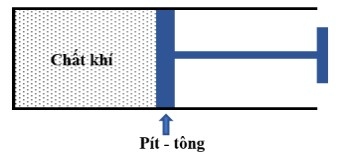
\includegraphics[width=0.3\linewidth]{../figs/D12-1-6}
	\end{center}
	\shortans{1,63 }
	\loigiai{
		Công khí thực hiện:
		$$A'=p\Delta V=\left(\SI{5.8E5}{\pascal}\right)\cdot\left(\SI{720E-6}{\meter^3}-\SI{500E-6}{\meter^3}\right)=\SI{127.6}{\joule}.$$
		Nhiệt lượng đã cung cấp cho khí:
		$$Q=\Delta U-A=\Delta U+A'=	\SI{1.63}{\kilo\joule}.$$
	}
\end{ex}
% ===============================================================
\begin{ex}
	Hiện nay, người ta có thể dùng các vỉ đá được làm nóng sẵn trong lò (tăng nội năng của vỉ đá) để nướng thức ăn. Giả sử, một vỉ đá có khối lượng $\SI{1.2}{\kilogram}$, nhiệt độ ban đầu là $\SI{28}{\celsius}$ được làm nóng trong lò có công suất $\SI{20}{\kilo\watt}$. Coi như toàn bộ năng lượng của lò cung cấp sẽ dùng để làm nóng vỉ đá. Biết rằng, để làm cho $\SI{1}{\kilogram}$ đá làm vỉ này tăng thêm $\SI{1}{\celsius}$ thì cần nhiệt lượng $\SI{5500}{\joule}$. Để vỉ đá đạt được nhiệt độ $\SI{1000}{\celsius}$ thì cần thời gian bao nhiêu phút? \textit{(Kết quả lấy đến hai chữ số sau dấu phẩy thập phân)}.
	\shortans{5.35 }
	\loigiai{
		$t=\dfrac{mc\Delta t}{\calP}=\dfrac{\left(\SI{1.2}{\kilogram}\right)\cdot\left(\SI{5500}{\joule/\kilogram\cdot\kelvin}\right)\cdot\left(\SI{1000}{\celsius}-\SI{28}{\celsius}\right)}{\SI{20E3}{\watt}}=\SI{320.76}{\second}\approx\SI{5.35}{\minute}.$
	}
\end{ex}
\Closesolutionfile{ans}
\begin{center}
	\textbf{-- HẾT --}
\end{center}